\documentclass[a4paper, 12pt]{article}
\usepackage[utf8]{inputenc}
\usepackage[T1]{fontenc}
\usepackage[scale=.8]{geometry}
\usepackage[french]{babel}
\usepackage{hyperref}
\usepackage{graphicx}
\usepackage{amsmath}
\usepackage{amssymb}

\title{Sécurité des données dans le cloud\\Doit-on se méfier du cloud ?}
\author{M1 Informatique}
\date{}

\begin{document}
  \maketitle
  \newpage
  \tableofcontents
  \newpage

  \section{Introduction}
    Aujourd'hui, une majorité de nos données personnelles, professionnelles,
    publiques comme privées, transitent par des services de stockage en ligne,
    des données qui peuvent aller de simples images publiques à des données
    confidentielles comme par exemple des données bancaires ou encore des
    documents secrets pouvant impacter l'intégralité d'un pays ou même du monde.

    Il est impératif de s'assurer de la sécurité de ses services de stockage,
    car les conséquences découlant de possibles négligeances pourraient avoir
    des effets catastrophiques.

    \subsection{Quelques statistiques}
      Un bon moyen de visualiser l'ampleur que le cloud à prit dans le monde est
      de l'illustrer par quelques statistiques
      \begin{itemize}
        \item Environ 94\% des entreprises utilisent des services de cloud.
        \item En 2025, selon les prévisions actuelles, 100 zettabytes de données
              devraient être stockées sur des services en ligne
              \footnote{Cela représente 10$^{23}$ octets de données soit
              10$^{11}$ disques dur de 1To}.
        \item En 2013, au total, seulement un exabyte de données était stocké
              sur des services de cloud\footnote{100 zettabytes = 100000
              exabytes}.
      \end{itemize}

      On peut voir par ces quelques statistiques que non seulement le nombre de
      données stockées en ligne est gigantesque, mais aussi qu'il croit très
      rapidement, il est donc nécessaire de se prémunir contre les risques
      potentiellement encourus.

    \subsection{Différents modèles de cloud}
      Les fournisseurs de services de cloud peuvent proposer différents modèles,
      proposant différents prestations que l'entreprise gère ou non pour
      l'utilisateur, les trois modèles généralement proposés sont les service
      d'infrastructure, de plateforme et de logiciel, respectivement nommés
      IaaS, PaaS et SaaS\footnote{aaS signifie as-a-Service, cette mention
      signifie qu'un fournisseur prend en charge la gestion du service et de
      certaines fonctionnalités pour les utilisateurs}. La différence entre ces
      trois modèles réside en le nombre de fonctionnalité dont le fournisseur
      laisse la gestion à l'utilisateur, le modèle IaaS est celui qui laisse le
      plus de fonctionnalités à la gestion de l'utilisateur, contrairement au
      modèle SaaS qui lui est géré complètement par le fournisseur. Néanmoins,
      aucun des modèles ne laisse au client la possibilité de gérer les
      fonctionnalités concernant l'accès réseau et le système de stockage
      utilisé.

  \section{Les failles de sécurité qui peuvent mener à un vol de données}
    L'inquiétude suscitée par le cloud est que ce genre de service hébèrge
    énormément d'utilisateurs. Si un attaquant réussi à pénétrer le cloud, il
    met la main sur les données de l'intégralité des personnes qui en font
    l'usage. Nous allons donc voir ce qui pourrait permettre à un attaquant de
    pouvoir voler les données stockées en ligne dans ce type de service.

    \subsection{Erreurs humaines et contrôle d'accès}
      La grande majorité des failles qui ont mené à des vols de données sur
      un cloud proviennent d'une erreur humaine, on peut citer parmis elles les
      défauts de configuration. c'est le modèle IaaS qui est mis en cause dans
      la plupart des cas. En effet, ce modèle de cloud est très flexible et
      permet aux utilisateurs de pouvoir configurer et gérer de nombreux aspects
      du cloud qu'ils utilisent, en les configurant potentiellement d'une façon
      trop peu sécurisée. Pour citer l'étude [AF2019], "\textit{about 99\% of
      misconfigurations go unnoticed by companies using IaaS}".
      \footnote{Traduction : Environ 99\% des erreurs de configurations ne sont
      pas remarquées par les entreprises utilisant le modèle IaaS}. \\

      Des erreurs peuvent aussi être commises losqu'il s'agit de l'accès des
      utilisateurs aux services et aux données stockées. Parfois un trop grand
      nombre de personne peut avoir accès à des données sensibles, par exemple
      au sein d'une entreprise, sans pour autant que cela soit nécessaire, cela
      découlant d'un manque de contrôle de ces accès. Laisser à trop de
      personnes l'accès à des données sensibles multiplie le risque d'attaque.
      On peut imaginer un attaquant extérieur qui pourrait vouloir pénétrer le
      stockage par ricochet en utilisant les utilisateurs concernés, mais aussi
      les utilisateurs eux-mêmes qui pourrait cacher un attaquant interne, il
      est donc nécessaire d'assurer un contrôle des accès rigoureux.

    \subsection{La gestion de la mémoire dans le cloud}
      À l'image d'un disque dur de taille normale, le cloud est un espace de
      stockage partagé par plusieurs systèmes et/ou utilisateurs, il est
      important de se concentrer sur la gestion de l'espace alloué à chacun.

      Un des problèmes cité page 3/4 de cette étude [VR2016] est le fait que la
      mémoire effacée peut être récupérée. En effet, \textit{"The resource
      allocated to a particular user may be assigned to the other user at some
      later point of time"}\footnote{Traduction : l'espace alloué à un
      utilisateur peut être assigné à un autre à un autre moment}. Les services
      de cloud marchent nécessairement avec un système d'allocation de mémoire
      dynamique en fonction de la requête d'espace de l'utilisateur. Les
      services n'ayant pas une quantité infinie de stockage, Un morceau de
      l'espace va surement être utilisé successivement par plusieurs
      utilisateurs différents. L'utilisateur de ce morceau de l'espace pourra
      donc potentiellement récupérer d'anciennes données effacées qui ne lui
      appartiennent pas.

      En effet, sur la plupart des machines, il est possible de récupérer des
      données qui ont été effacés. Les données ne sont en réalité pas rééllement
      effacées tant que le disque ou le dispositif de stockage n'a pas réécrit
      d'autres données par dessus. Si un utilisateur dispose d'un morceau de la
      plage mémoire allouée précedémment à un autre utilisateur, il pourra donc
      tenter de les récupérer. \\

      Un autre problème posé par le partage massif du cloud est la fragmentation
      de la mémoire. En effet, un problème pourraient résider dans la mauvaise
      ségmentation de la mémoire. Ceci pourrait permettre l'accès au même
      morceau de mémoire par plusieurs personnes, et un utilisateur pourrait
      voler des données à un autre, ou même récupérer des données supprimées
      comme dit plus haut.

    \subsection{Risques physiques}
      Les clouds sont des espaces de stockages, il est aussi nécessaire de
      considérer les menaces liées aux supports de stockages physiques des
      données comme les centres de stockages. Un attaquant pourrait très bien
      décider de pirater physiquement un centre de données, il est donc aussi
      nécessaire de se prémunir des risques physiques liées à l'intégrité des
      données stockées dans le cloud.

  \section{Anticipation et prévention des risques}
      L'identification des risques liés à une installation dans le cloud est
      primordiale car elle permet de pouvoir réfléchir à des solutions pour
      anticiper les attaques et les solutionner. Puisqu'il existe de nombreux
      risques dont une partie on été traités dans la partie précédente, il
      existe un grand nombre de méthodes et de solutions pour les anticiper
      et les éviter.

      \subsection{Un aspect social}
      Le domaine de l'ingénieurie sociale est en hausse car il s'agit très
      certainement de la méthode la plus simple et non moins efficace pour
      obtenir l'accès à des données ou des services illégitimement. Il est
      crucial pour quiconque s'intéresse à la technologie du cloud et d'autant
      plus pour les entreprises de se former et de former l'ensemble des
      équipes au risques bien réels auxquels ils peuvent faire face dans leur
      quotidien. \\

      Pour une entreprise du cloud il est aussi nécessaire de définir
      clairement des règles de conduite pour l'ensemble du personnel afin
      d'éviter au maximum les failles de sécurité sensibles à l'ingénieurie
      sociale. D'autant plus que ce sont des failles critiques qui peuvent
      parfois déboucher sur des pertes de données conséquentes. \\

      Pour revenir sur un court exemple, on pourrait reparler de l'attaque 
      subie par l'entreprise Uber en 2022 qui à eu lieu suite à un fait 
      d'ingénieurie sociale qui a permis à un attaquant l'accès à l'un des 
      comptes administrateur de l'entreprise. Avec une politique de conduite 
      plus stricte et une mise en garde sur les risques, l'attaque aurait pu 
      être détectée plus tôt et surtout évitée. \\

    \subsection{Sur le plan physique}
      Les clouds étant des espaces de stockages numériques auxquels un
      utilisateur à très peu voir pas du tout d'accès sur le plan physique.
      Qu'il soit un particulier ou une entreprise, lorsqu'un utilisateur
      prévoit l'utilisation d'un service cloud, il devient alors nécessaire de
      procéder à une étude des risques physiques liés au fournisseur de
      ce service et à la politique de sécurité qu'il applique au sein de ses
      infrastructures. Y a-t-il de la surveillance, des contrôle d'accès ou
      d'autres mesures permettant de garantir un accès limité au site ? Il
      existe notamment certaines certifications qui peuvent être utilisées dans
      ce but comme la certification ISO 9000\footnote{Certification délivrée
      par l'organisme ISO selon un certains nombres de critères comme
      l'organisation, les clients, les données, les systèmes etc.} ou SAS 70
      \footnote{State on Auditing Standards no. 70, remplacée par SSAE16. Il
      s'agit d'une certification spécialisée pour les centre de données} par
      exemple. De plus, certains fournisseurs de cloud ont une politique de 
      confidentialité concernant l'emplacement et les spécificités de leurs 
      datacenters afin de se prémunir contre les menaces. \\

      Tout cela étant dit, une perte de donnée ou une rupture d'accès à un
      service dans le cloud ne provient pas toujours d'une action volontaire
      d'un ou plusieurs individus. C'est pour cela que le contrôle d'accès et
      la surveillance ne suffisent pas à garantir la sécurité des données ou
      du service. Il est aussi nécessaire de se prémunir des risques liés à des
      catastrophes naturelles comme les incendies, les inondations ou bien
      plus simplement des coupures de courant par exemple. Cela peut-être
      effectué en prévoyant une redondance des données grâce à des sauvegardes
      régulières chiffrées et stockées dans d'autres infrastructures. Dans le
      cadre d'un service qui outrepasse le simple stockage de données, il est
      aussi nécessaire de prévoir une redirection du service vers une autre
      plateforme fonctionnelle. Cela parmet d'éviter les interruptions de
      service pour des applications cloud qui y seraient sensibles.

    \subsection{Sur le plan technique}
      L'une des difficultés d'un système dans le cloud réside dans les 
      responsabilités d'actions ambiguës. En effet, si l'on considère les 
      trois types de cloud, à savoir IaaS, PaaS et SaaS, il est parfois 
      difficile pour un utilisateur de comprendre quelles actions sont à 
      sa charge. \\

      Dans le cas d'un cloud SaaS, l'utilisateur a très peu de contrôle sur 
      la manière dont les choses vont fonctionner à l'intérieur de sa machine.
      En réalité, l'ensemble de la configuration système et logicielle sur 
      laquelle va reposer son service est aux mains du fournisseur d'accès.
      Cela a de nombreux avantages puisque l'ensemble des côuts d'architecture
      et de sécurisation sont finalement gérés par le fournisseur de service qui 
      garantit en plus de cela un niveau de sécurité en théorie plus 
      intéressant du fait de son expertise sur ses propres systèmes. Un point 
      crucial et pourtant évident reste cependant aux mains de l'utilisateur. 
      Il s'agit du choix de moyens d'authentification aussi sécurisés que 
      possible, quite à utiliser de l'authentification multi-factorielle voir
      de l'expiration de mots de passes. Il s'agit là du seul point vraiment 
      sensible de cette configuration. \\

      L'utilisation d'un cloud de type PaaS n'est pas très différente de 
      celle d'un SaaS d'un point de vue sécurité informatique. L'utilisateur 
      n'aura pas non plus à s'occuper de la configuration système et logicielle
      qui reste ainsi au fournisseur. Cependant un utilisateur de ce type de 
      cloud devra se charger de la sécurité des applications qu'il décidera de 
      déployer sur le système ainsi que de leurs services associés comme les 
      bases de données par exemple. La gestion de la sécurité de ces 
      applications peut être déléguée à des experts, ou dans le cas d'une
      entreprise suffisamment importante, elle sera très certainement gérée 
      par l'un des services de l'entreprise en question. \\

      Même si l'utilisation d'un cloud SaaS ou Paas semble idéale d'un point 
      de vue sécurité pour la plupart des utilisateurs, il ne s'agit cependant 
      pas d'une solution universelle puisque certains utilisateur particuliers 
      ou entreprises ont besoin de plus de flexibilité. Plus de flexibilité 
      implique inévitablement plus de responsabilités. Ainsi sur un cloud de 
      type IaaS, l'utilisateur se trouve pratiquement sur une machine vide sur 
      laquelle il va devoir installer un système d'exploitation et procéder à 
      sa configuration. Par dessus ce système, il faut ensuite installer les
      logiciels et applications nécessaires. A ce moment là, sécuriser le 
      système se rapproche finalement de ce que l'on connaissait par le passé
      quand chaque enntreprise disposait de sa propre installation physique. \\

      La complexité de la sécurisation d'un système cloud réside plus souvent
      du côté du fournisseur de cloud tel qu'Azure, AWS, OVH et beaucoup 
      d'autres. De ce côté là chaque fournisseur développe ses propres 
      technologies de sécurité. Les technologies et outils sont nombreux mais
      on peut citer les systèmes d'authentification basés sur les privilèges, 
      les systèmes de monitoring et d'analyse du système ou bien des logiciels 
      de chiffrement des données par exemple. \\

      Malgré les solutions qui existent aujourd'hui, la sécurité du cloud
      reste un des enjeux de ces prochaines années car il est encore difficile
      d'assurer une installation fiable de manière pérenne sans déployer de
      gros moyens financiers et humains.

  \section{L'avenir de la sécurité dans le cloud avec l'IA ?}
    Depuis la crise sanitaire causée par le COVID-19 en 2020, les organisations
    accélèrent leurs transformations numériques, en trouvant de nouvelles façons
    de travailler et de communiquer. La sécurité des organisations évolue petit
    à petit chaque jour, et les cybercriminels adaptent également leur façon
    d'attaquer les systèmes. Avec l’émergence de l'intelligence artificielle
    dans la cybersécurité, le système immunitaire des organisations peut
    fonctionner de manière autonome et s'adapter aux conditions inconnues et
    imprévisibles de chaque système et attaque.

    \subsection{La prévention par l'IA}
      Avec les bonnes données, les solutions Machine Learning peuvent
      prédire avec précision les événements futurs. Pour que cela fonctionne,
      les experts doivent recueillir beaucoup d'informations et les utiliser
      pour créer des modèles prédictifs. Ces données montrent donc comment
      divers événements pourraient se dérouler. En cybersécurité, les
      organisations peuvent comprendre les menaces potentielles et prédire ce
      qui pourrait arriver grâce au Machine Learning. \\

      Pour l’instant, ces systèmes ne sont pas encore assez développés.
      Néanmoins, les perspectives de développement de l’IA\footnote{Intelligence
      Artificielle (AI en anglais)} préventive en cybersécurité se décomposent
      en deux types. Le premier type d'IA a besoin d’une grosse banque
      d'informations concernant les différentes attaques contre les
      organisations similaire qui ont déjà eu lieu. L'IA peut alors effectuer
      une évaluation précise des risques pour une entreprise donnée. Le deuxième
      type d’IA est beaucoup plus complexe, car celle-ci se repose sur le
      travail d’un White-Hat\footnote{Pirate éthique expert en cybersécurité qui
      réalise des tests d'intrusion et d'autres méthodes de test afin d'assurer
      la sécurité des systèmes d'information d'une organisation} en utilisant
      les ressources et reproduisant les attaques. Le principe ici est
      d’automatiser les tests d’intrusions réalisées par ces White-Hat afin de
      déceler les failles présentes dans un cloud.

    \subsection{La protection par l'IA}
      Les modèles actuels d'IA peuvent lutter en permanence contre les
      menaces. Beaucoup d’entreprises s'appuient sur ces outils pour la sécurité
      dans le cloud afin de prendre des mesures sans interruption. Une des idées
      communes sur systèmes d'IA est qu'ils peuvent répondre intelligemment aux
      attaques et ça instantanément. Cependant, il s'agit d'une idée fausse pour
      deux raisons principales. La première est que ces systèmes font uniquement
      des suggestions aux administrateurs, mais eux seul peuvent prendre des
      mesures lors d'une attaque. Ainsi, ces technologies ne font que suivre des
      règles simples et préalablement programmées. Ensuite, même si l’IA dans le
      cloud peut agir directement sur les systèmes, il existe toujours des
      limites. Bien cette technologie puisse empêcher certains utilisateurs
      d'accéder à certaines zones, les privilèges donnés sont généralement
      limités pour éviter toute mauvaise décision. \\

      L’intégration de l’IA dans un cloud pour la cybersécurité affecterait
      directement les systèmes de l’organisation ce qui comporte des risques
      importants. Si le système d'IA vient à prendre de mauvaises décisions, il
      pourrait éventuellement bloquer les utilisateurs et les systèmes, ce qui
      impacterait fortement les organisations.

    \subsection{Comment ça marche ?}
      Avant de prendre des mesures défensives, l’IA doit analyser le
      comportement de l’attaquant en réalisant une analyse préventive. Le
      système doit étudier premièrement les projections d’attaque, c’est-à-dire,
      est-ce qu’il va y avoir potentiellement un attaquant. Ensuite, il faut
      reconnaitre les intentions de celui-ci en trouvant son but grâce à des
      paternes déjà connu. Enfin, l’IA doit reconnaître le type d’attaque, quand
      et comment va-t-elle se passer et les mesures qu’elle doit mettre en œuvre
      pour éviter ces attaques. Ces préventions passant par la perception, la
      compréhension et la projection de ses attaques utilisent 3 types
      d’approche mathématique, le modèle discret, le modèle continu et le
      Machine Learning. Ces 3 approches permettent de cibler les différents
      paramètres d’une attaque et son type. On retrouve notamment dans ces
      approches, l’utilisation de graphes orientés pondérés pour prédire avec
      une certaine probabilité le prochain type d’attaque en fonction de la
      précédente, comme on peut le voir dans la figure \ref{fig:1}. \\

      \begin{figure}[h]
        \centering
        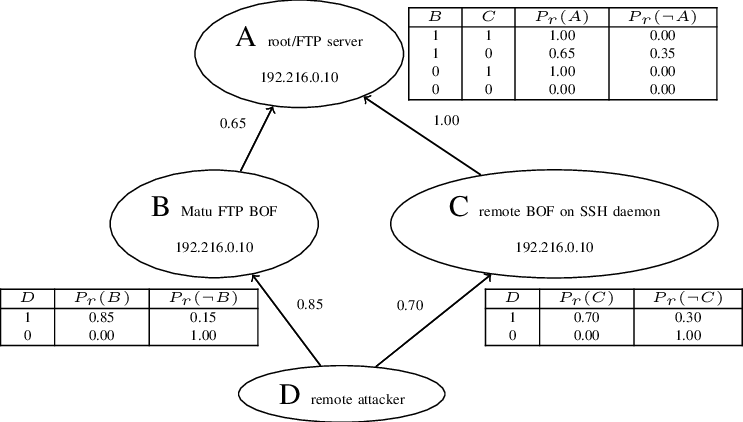
\includegraphics[scale=.4]{img/attackgraph.png}
        \caption{Graphe bayesien d’une attaque potentielle. Source : [MJEP18]}
        \label{fig:1}
      \end{figure}

      L’IA s’assure plusieurs fois qu’il s’agit vraiment d’une attaque
      malveillante menaçant l’intégrité de l’entreprise. Une fois la menace et
      le type d’attaque identifié, il ne reste plus qu’à prendre des mesures
      contre cette attaque. L’IA sera limité aux accès que l’administrateur lui
      aura attribués. Celle-ci pourrait par exemple pouvoir bloquer la connexion
      aux serveurs pour une certaine adresse IP ou encore une certaine machine
      interne probablement infectée.

    \subsection{Solution viable ou non ?}
      Malgré de nombreuses idées fausses sur ce que l'IA peut réellement
      faire pour améliorer les systèmes de sécurité, cet outil joue un rôle
      important dans l'amélioration de la sécurité du cloud. Il a également de
      grandes perspectives d’évolution. L’IA pourrait contribuer à la pénurie de
      compétences en cybersécurité qui donne l'opportunité aux pirates de mener
      des activités frauduleuses. Alors que cette technologie stimule déjà
      l'innovation et la protection contre les menaces, l'IA pourrait réduire
      les efforts des professionnels en cybersécurité et automatiserait le
      processus de protection. Alors que les pirates continuent d'améliorer
      leurs attaques, la mise en œuvre de l'IA dans la sécurité du cloud
      deviendra plus efficace. Toutes les cyber-opérations peuvent être
      entièrement automatisées avec une intervention humaine minimale. \\

      Actuellement, le problème de l’IA pour la cybersécurité dans le cloud est
      que les organisations l’utilisant se repose trop sur elle, croyant que le
      système pourrait détecter et arrêter toutes les attaques. Comme dit
      précédemment, ces système sont encore trop sous-développé. Au lieu de
      s'appuyer sur l’IA, les sociétés devraient se concentrer sur
      l'amélioration des plates-formes de sécurité cloud pour fournir des
      réponses optimales tout en continuant à investir dans ces systèmes jusqu’à
      atteindre des résultats asses satisfaisant pour se reposer entièrement sur
      ceux-ci.

  \section{Conclusion}

  \section{Bibliographie}
    \begin{itemize}
      \item \href{https://www.sciencedirect.com/science/article/pii/S1877050916315812}{[VR2016] A Study on Data Storage Security Issues in Cloud Computing} : \url{https://www.sciencedirect.com/}
      \item \href{https://www.mcafee.com/enterprise/en-us/assets/reports/restricted/rp-cloud-adoption-risk-report-iaas.pdf}{[AF2019] Cloud-Native: The Infrastructure-as-a-Service (IaaS) Adoption and Risk Report} : \url{https://www.mcafee.com/}
      \item \href{https://www.researchgate.net/publication/327449459_Survey_of_Attack_Projection_Prediction_and_Forecasting_in_Cyber_Security}{[MJEP18] Projection, prédiction et anticipation d'attaque dans la sécurité informatique} : \url{https://www.researchgate.net}
    \end{itemize}

  \section{Webographie}
    \begin{itemize}
      \item \href{https://www.cloudwards.net/cloud-computing-statistics/}{Quelques statistiques à propos du cloud} : \url{https://www.cloudwards.net}
      \item \href{https://parachute.cloud/cloud-computing-statistics/}{Différentes statistiques sur l'utilisation et la présence du cloud} : \url{https://parachute.cloud/}
      \item \href{https://www.globaldots.com/resources/blog/how-much-is-stored-in-the-cloud/}{Données datant de 2013 sur la taille du cloud} : \url{https://www.globaldots.com}
      \item \href{https://aws.amazon.com/fr/types-of-cloud-computing/}{Différents types de cloud et de services proposés} : \url{https://aws.amazon.com}
      \item \href{https://www.redhat.com/fr/topics/cloud-computing/what-is-iaas}{Le type de service IaaS et comparaisons avec PaaS et SaaS} : \url{https://www.redhat.com/}
      \item \href{https://www.javatpoint.com/cloud-deployment-model}{Différents types de déploiement des services de cloud} : \url{https://www.javatpoint.com/}
      \item \href{https://www.cyberuniversity.com/post/la-securite-dans-le-cloud-principaux-risques-et-challenges}{Principaux risques encourus en stockant sur le cloud} : \url{https://www.cyberuniversity.com/}
      \item \href{https://www.techtarget.com/searchdisasterrecovery/definition/data-recovery}{Récupération de données effacées} : \url{https://www.techtarget.com/}
      \item \href{https://www.runtime.org/recoverability.htm}{Autres données sur la récupération de données effacées} : \url{https://www.runtime.org/}
      \item \href{https://www.techniques-ingenieur.fr/actualite/articles/la-securite-dans-le-cloud-une-approche-fournisseur-basee-sur-les-risques-15550/}{Différents risques liés cloud} : \url{https://www.techniques-ingenieur.fr/}
      \item \href{https://www.magic.fr/cloud-public-les-erreurs-de-configuration-sont-extremement-frequentes/}{Erreurs humaines, défauts de configuration} : \url{https://www.magic.fr/}


      \item \href{https://www.rcarre.com/blog/intelligence-artificielle-auto-apprenante-pour-le-cloud-and-saas/}{IA auto apprenante pour le cloud et particulièrement le modèle SaaS} : \url{https://www.rcarre.com}
      \item \href{https://itsocial.fr/partenaires/oracle-partenaire/tribunes-oracle/securite-du-cloud-entre-intelligence-artificielle-et-responsabilite-humaine/}{Sécurité entre IA et responsabilite humaine} : \url{https://itsocial.fr}

    \end{itemize}
\end{document}
